\documentclass{article}
\usepackage[finnish]{babel}
\usepackage{1inchmargins}
%\usepackage[iso]{isodate}
\usepackage{hyperref}
\usepackage{color}
\usepackage[utf8]{inputenc}
\usepackage[T1]{fontenc}
\usepackage{booktabs}
\usepackage{amsmath}
\usepackage{graphicx}
\renewcommand{\familydefault}{\sfdefault}
\renewcommand{\tabcolsep}{8pt}


\hypersetup{
    colorlinks=true,
    urlcolor=blue,
}

\newcommand{\surl}[1]{{\small \url{#1}}}

\begin{document}


\centerline{\sf \Huge AstroTortilla käyttöohje}
\centerline{Viimeisin päivitys: \today}

\tableofcontents

\setlength{\parindent}{0pt}
\setlength{\parskip}{2ex}

\newpage

\section{Johdanto}

\emph{Astrometrinen ratkaisu sokkona} tunnistaa minkä tahansa tähtikuvan 
sijainnin taivaalla tietämättä kuvasta mitään etukäteen. \emph{AstroTortilla} 
hyödyntää sokkoa ratkaisua kertoakseen seurantajalustallesi mihin päin kaukoputkesi
osoittaa. Tämän ansiosta tähtikuvaus tietokoneella muuttuu helpommaksi kuin koskaan - ilman lisähintaa.

AstroTortilla yhdistää ohjelmistot joita jo käytät (kameraa ja jalustaa käskyttävät ohjelmat) 
ja laittaa ne juttelemaan kuvakenttiä ratkaisevan ohjelman kanssa.

Vaikka tekisit miten pitkiä \emph{GoTo}-käännöksiä tahansa taivasta pitkin, 
AstroTortilla keskittää haluamasi kohteen automaattisesti \emph{täsmälleen} 
keskelle kuvaruutua -- vaikka jalustasi kalibrointi olisi miten epätarkka hyvänsä.

Kuvakenttien sijainnin ratkaisemista hyödyntämällä myös napasuuntaus sujuu helposti, parissa minuutissa.
Anna AstroTortillan katsella hetki ympärilleen, niin ohjelma kertoo sinulle napasuuntausvirheesi asteissa.
Joudut kuitenkin itse kääntelemään suuntausruuveja!

Paikallisen ruokavalion perustaa, \emph{Meksikolaista tortillaa} käytetään
käärimään liha ja kasvikset yhdeksi helposti syötäväksi paketiksi.
\emph{AstroTortilla} käärii yhteen tarvittavat tietokoneohjelmat herkulliseksi
yöpalaksi tähtitaivaan alla.
 

\section{Tuetut tietokoneohjelmat ja laitteistot} 
\subsection{Kameran ohjaus}

AstroTortillaa käyttääksesi tarvitset tavan siirtää kuvia kamerastasi tietokoneelle. Tuettuja keinoja ovat tällä hetkellä
\begin{itemize}
\item \textbf{{MaxIm DL}} 
\item \textbf{{Nebulosity 2/3}} 
\item \textbf{{Astro Photography Tool}} 
\item \textbf{{Ruutukaappaus}} mistä tahansa muusta ohjelmasta (esim. \emph{PHD Guiding} tai \emph{BackyardEOS})
\item Suora yhteys kameraan \textbf{ASCOM}-ajurilla
\item \textbf{Tiedoston avaaminen kovalevyltä} manuaalisesti
\end{itemize}

Tulevaisuudessa mukana on toivottavasti myös varta vasten rakennettu tuki \emph{BackyardEOS}:lle ja muille tähtikuvausohjelmille. Jos haluat toteuttaa tuen lempiohjelmistollesi, ota yhteyttä!

\subsection{GoTo-jalustan ohjaus}

AstroTortilla tukee kaikkia \hbox{\textbf{ASCOM-rajapinnan}} kautta tietokoneohjattavia
seurantajalustoja. Ohjelmaa kehitetään ja testataan Komakalliolla käyttäen 
Sky-Watcherin HEQ5- ja EQ6-jalustoja EQMOD-ohjelman avulla.

ASCOM rajoittaa ohjelman toimivuuden Windows-koneille. 

\subsection{Astrometrinen ratkaisu}

Astrometrinen ratkominen on laji, jossa pyritään tunnistamaan tähtien muodostamia kuvioita.
Kun oikeat tähdet on ratkaistu, voidaan niiden avulla päätellä kuvan atrkat koordinaatit taivaalla,
kuvakentän korkeus, leveys ja kiertokulma taivaan koordinaattiakseleihin nähden, 
kuvan pikseleiden mittakaava taivaalla kaarisekunneissa. Mikäli kameran pikseleiden 
fyysinen koko tunnetaan, voidaan laskea myös kaukoputken polttoväli tarkasti.

Normaalisti kuvakentän ratkaisu vaatii tähtikatalogin eli tietokannan tähtien sijainneista sekä 
karkea arvio siitä, minne päin kamera osoittaa.

\subsubsection{Astrometry.net}

Vallankumouksellisen mullistavassa Astrometry.net-projektissa kehitellään
työkalua, jolla saadaan astrometrinen ratkaisu mille tahansa tähtikuvalle
\emph{ilman mitään etukäteistietoa} kuvasta. Projektin ohjelmisto, algoritmit 
ja lähdekoodi ovat vapaasti saatavilla. Ratkaisun löytyminen nopeasti täysin sokkona
perustuu siihen, että suurin osa raskaasta laskennasta tehdään etukäteen luetteloimalla
neljän tähden muodostamia kuvioita ja lajittelemalla niitä nokkelalla tavalla valtaviin
tietorakenteisiin.

Astrometry.net on tätä kirjoitettaessa betatestausvaiheessa. Projektin 
online-käyttöliittymä löytyy osoitteesta \surl {http://nova.astrometry.net/}.
Astrometry.netiä voi myös ajaa paikallisesti Linux, Unix, MacOS tai
Cygwin for Windows -ympäristöissä.

AstroTortilla käyttää Astrometry.netin paikallista versiota Cygwin-ympäristön avulla.
Asentaminen on tehty erityisen helpoksi -- AstroTortillan asennusohjelma lataa ja 
asentaa kaiken tarvittavan automaattisesti.

Tulevaisuudessa AstroTortilla saattaa tukea myös kuvien ratkaisemista internet-käyttöliittymällä
niille, joiden kuvauslaitteisto on vaatimaton kovalevytilan ja laskentatehon, mutta ei nettiyhteyden suhteen.
Tällä hetkellä se on kuitenkin mahdotonta Astrometry.netin puolivalmiin online API:n takia.

\newpage

\section{AstroTortillan asennus}

Asentaminen on helppoa, sillä AstroTortillan asennusohjelma sisältää nykyään
kaiken tarvittavan. Koneellesi asennetaan automaattisesti Cygwin-ympäristö toimivalla
toimivalla astrometry.net-versiolla. Asennusohjelma lataa myös ratkaisijaohjelman tarvitsemat
indeksitiedostot (tähtiluettelot). Voit räätälöidä haettavien tiedostojen määrän oman kaukoputkesi näkökentälle sopivaksi.

Cygwin-asennus vie noin 300 megatavua tilaa kiintolevyltäsi. Sen lisäksi että Cygwin on
välttämätön Linux-pohjaisen astrometry.netin käyttämiseen Windowsissa, se tarjoaa 
näppärän kokoelman Linux-tyylisiä komentorivityökaluja joista saatat hyötyä tai sitten et.
AstroTortillan käyttämiseen et kuitenkaan tarvitse komentoriviä.

Indeksitiedostot eli tähtiluettelot sen sijaan vievät vielä enemmän tilaa. 
Kameralinsseillä ja lyhyillä linssiputkilla otettujen kuvien ratkaisemiseen 
riittää noin yhden gigatavun kokoinen paketti indeksejä. Kapeammat kuvakentät 
(eli pidemmät polttovälit) vaativat lisää indeksitasoja. Jokainen uusi taso on 
kaksi kertaa edellistä suurempi ja koko täydellinen indeksipaketti vie noin 25 gigatavua tilaa.

Viittä kaariminuuttia pienempien kenttien ratkominen ei ole mahdollista.

\subsection{Lataa asennusohjelma}

Asennusohjelma löytyy osoitteesta \surl{http://astrotortilla.sourceforge.net/}. 
Tarkista että lataat uusimman version. Tallenna ja käynnistä \texttt{AstroTortilla-<versio>.exe}. 

Jos tiedät mitä 64-bittisyys tarkoittaa, kokeile x64-versiota.

\subsection{Valitse asennettavat osat}

Klikkailtuasi läpi asennuksen alun, valitse mitä haluat asentaa.

\begin{description}
\item [Asenna AstroTortilla, Cygwin, astrometry.net ja indeksit (Oletus)] \hfill \\
Oletusvalinta. Valitse tämä ensimmäisellä kerralla asentaaksesi kaiken tarvittavan.

\item [Asenna AstroTortilla, Cygwin, astrometry.net ilman indeksejä]\hfill \\
Use this option if you don't yet know your Field of View, or want to get the index files later for some other reason.

\item [Asenna vain AstroTortilla] \hfill \\
Tällä voit päivittää vanhentuneen tai poistetun AstroTortillan koskematta toimivaan Astrometry.net-asennukseen Cygwinissä.

\item [Lisää uusia astrometrisiä indeksejä] \hfill \\
Jos et asentanut indeksejä ensimmäisellä kerralla tai haluat valita lisää tasoja, valitse tämä.

\item [Päivitä Cygwin, astrometry.net ja asenna indeksejä] \hfill \\
Kun Astrometry.net päivittyy, teemme uuden Cygwin-version. Valitse tämä päivittääksesi.
\end{description}


\subsection{Indeksien valinta}

{\scriptsize \textbf{Kärsimätön?} Jos kuvaat alle 1000 mm polttoväillä, hyppää yli matematiikasta ja lataa tasot 4004--4019! (n. 2 GB)}

Seuraavaksi valitse mitkä indeksitiedostot haluat ladata. Valinta riippuu kuvauslaitteistosi näkökentästä.

Voit käyttää nettilaskuria näkökentälle tai arvioida koon tällä kaavalla:
\[
\text{Näkökenttä (\ensuremath{^\circ})}=\frac{57.3\times\text{Kennon koko}}{\text{Polttoväli}}
\]
Valitse Kennon koko ja Polttoväli samassa yksikössä, esim. 17 mm ja 1200 mm. Kennon kooksi voit valita minkä tahansa mitan (korkeus, leveys, lävistäjä), tarvitset vain suuruusluokan. Muuntaaksesi tuloksen asteista kaariminuuteiksi, kerro 60:llä.

Astrometry.net etsii kuvistasi neljän tähden kuvioita eli \emph{quadeja}. Quadit ovat kooltaan 10\%--100\% kuvasi koosta. Valitse tasoja, jotka sisältävät tämän suuruusluokan Quadeja.

\textbf{Esimerkki:} Arvoilla 17 mm ja 1200 mm kuten yllä, näkökenttä on noin $0.8^\circ \approx 50'$. Tasot 4004--4009 kattavat quadeja $8'$ ja $60'$ väliltä. Muutama megatavu lisää ei tunnu missään, joten otetaan kaikki 4004:stä 4019:ään asti. Nämä vievät yhteensä noin 2 gigatavua tilaa.

\begin{table}[!h]
\centering
\begin{tabular}{r r r @{ } c @{ } l r @{ } c @{ } l} \toprule
Indeksitaso 	& Koko (Mt) & \multicolumn{3}{r}{Quadit ($^\circ$)} & \multicolumn{3}{r}{Quadit (')} \\ \midrule
4000 & 11 Gt 	&  	&--& 		& 2 	&--&	2.8\\
4001 & 7 Gt 	&  	&--&  	& 2.8	&--&	4\\
4002 & 4 Gt 	&  	&--&  	& 4 	&--&	5.6\\
4003 & 2	Gt 	&  	&--&  	& 5.6	&--&	8\\
4004 & 960  	&  	&--&  	& 8 	&--&	11\\
4005 & 470  	&  	&--&  	& 11 	&--&	16\\
4006 & 230  	&  	&--&  	& 16 	&--&	22\\
4007 & 115  	&    	&--&  	& 22 	&--&	30\\
4008 & 62  		& 0.5 &--& 0.7	& 30 	&--&	42\\
4009 & 31  		& 0.7 &--& 1	& 42 	&--&	60\\
4010 & 15  		& 1 	&--& 1.4	& 60 	&--&	85\\
4011 & 5.6  	& 1.4	&--& 2	& 85 	&--&	120\\
4012 & 2.8  	& 2 	&--& 2.8	& 120 &--&	170\\
4013 & 1.4  	& 2.8	&--& 4 	& 170	&--&	240\\
4014 & 0.7  	& 4	&--& 5.6	&		&--&		\\
4015 & 0.4  	& 5.6	&--& 8 	&		&--&		\\
4016 & 0.2  	& 8	&--& 11	&		&--&		\\
4017 & 0.09  	& 11	&--& 17	&		&--&		\\
4018 & 0.06  	& 17	&--& 23	&		&--&		\\
4019 & 0.04  	& 23	&--& 33	&		&--&		\\ \bottomrule
\end{tabular}
\end{table}

Jos palaat asennuksen tähän kohtaan myöhemmin hakeaksesi lisää tasoja, voit jättää laajimman indeksin 4019:ksi. 
AstroTortilla tietää mitkä indeksit ovat jo asennettuna ja hakee vain puuttuvat.

\subsection{Asennuksen viimeistely}

Seuraavaksi klikkaile asennus loppuun. Nyt voit käynnistää AstroTortillan ja testailla kuvien ratkomista vaikka vanhoilla ruuduillasi.
Voit myös yhdistää ASCOM-jalustasimulaattoriin ja katsella planetaario-ohjelmassa kuinka AstroTortilla kääntää jalustan kuvan sijaintia kohti.

\section{AstroTortillan käyttö}

\subsection{Pääikkuna}

AstroTortillan pääikkuna koostuu neljästä paneelista: Jalusta (Telescope), Kamera (Camera), Ratkoja (Solver) ja Toiminnot (Actions).

\begin{figure}[h!]
\centering
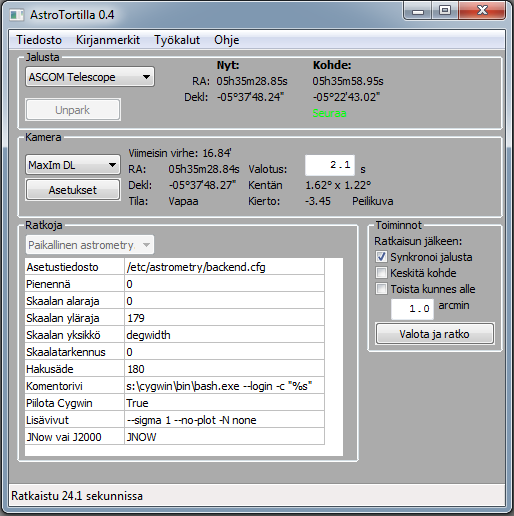
\includegraphics[width=0.72\textwidth]{Tortilla-v04-screen-fi.png}
\end{figure}

\subsubsection{Jalusta}

Valitse pudotusvalikosta \textbf{ASCOM Telescope}, jonka jälkeen valitse oma jalustasi (voit myös kokeilla ASCOM-simulaattoria).

Toimiakseen järkevästi jalustasi ASCOM-ajurin on syytä toimia ns. hubina, 
eli mahdollistaa useamman ohjelman olla yhteydessä ajuriin yhtäaikaisesti.
Jos näin ei ole, tutustu Plain Old Telescope Handset (POTH):iin.

\subsubsection{Kamera}

Valitse miten yhdistät kamerasi tietokoneeseen. Valmis tuki löytyy seuraaville ohjelmille: \textbf{Astro Photography Tool}, \textbf{MaxIm DL} ja \textbf{Nebulosity}. 

Maxim DL:lle ja Nebulositylle voit asettaa AstroTortillan valotuksissa käytettävän suodattimen ja binnausasetuksen. Nebulosityn käyttäjien kannattaa lisäksi asettaa kuvaushakemiston palautus, sillä AstroTortilla ei pysty lukemaan Nebulosityn tämänhetkistä kuvaushakemistoa. Tämän helpottamiseksi AstroTortilla tarjoaa kaksi makroa päivämäärän syöttämiseksi, \textit{\%(date)s} on nykyinen tarkka päivämäärä ja \textit{\%(night)s} vaihtaa päivää keskipäivällä. Molempien formaatti on YYYY-MM-DD. AstroTortillassa ei yleensä tarvitse valita mitä kameraa Nebulosity käyttää.

Jos käytät jotain muuta ohjelmaa, valitse \textbf{Ruutukaappaus} (Screen capture). Annetut asetukset toimivat PHD Guidingille. 
Muille ohjelmille saat itse ronkkia asetukset kuntoon.

Manuaaliseen käyttöön tai sisätiloissa testaamista varten valitse \textbf{Avaa tiedosto} (File Open dialog). AstroTortilla pyytää sinua avaamaan kuvan aina halutessaan "valottaa" kameralla.

Voit lisäksi yhdistää kameraan suoraan \textbf{ASCOM}-ajurilla.

AstroTortilla ei luotettavasti osaa käynnistää kuvausohjelmia, ja muutenkin on suositeltavaa, että olet ottanut yhden valotuksen käyttämälläsi kuvausohjelmalla varmistaaksesi laitteiston toiminnan ja tarkennuksen.

\subsubsection{Ratkoja}

Tässä ainoa vaihtoehto on paikallinen astrometry.net. Voit muuttaa ratkaisijan asetuksia asetustaulukossa.

\subsubsection{Toiminnot}

Tässä voit valita mitä onnistuneen valotuksen ja ratkaisun jälkeen tapahtuu.
\begin{description}
\item[Synkronoi jalusta (Sync Scope)] \hfill \\
Kerro jalustalle, että se osoittaa ratkaistuihin koordinaatteihin.
\item[Keskitä kohde] \hfill \\
Käännä jalusta sinne, mihin GoTo \emph{luuli} osoittavansa aiemmin.
\item[Toista kunnes alle ... arcmin ] \hfill \\
Toista kuvaus, ratkaisu ja kääntyminen kunnes kohde on täsmälleen keskellä (valitsemallasi tarkkuudella).
\end{description}

\subsection{Normaali käyttötapa}

Yhdistettyäsi laitteesi ja ohjelmasi, käännä jalusta johonkin kohteeseen 
jalustasi ohjausohjelmalla tai jollain tähtikarttaohjelmalla.
Kääntymisen jälkeen Kohde (Target) -kenttä näyttää valitsemasi kohteen koordinaatit. Nyt (Current) -kenttä näyttää samat koordinaatit,
koska toistaiseksi jalusta luulee olevansa täydellinen. Näin ei kuitenkaan yleensä ole.

Ruksi haluamasi valinnat Toiminnot-paneelista (esim. kaikki kolme) ja valitse valotusaika Kamera-paneelissa.
Paina Valota ja ratko (Capture and Solve).

AstroTortilla valottaa nyt kuvan ja toimittaa sen kameralta ratkaisijalle. Onnistuneen
ratkaisun jälkeen AstroTortilla tietää tarkalleen, mihin kaukoputki \emph{todella} osoittaa ja näyttää
ratkaistut koordinaatit Kamera-paneelissa.

Jos ruksit \emph{Synkronoi jalusta}, todelliset koordinaatit näkyvät nyt myös Nyt-kentässä ja jalustasi on GoTo-kalibroitu yhdellä pisteellä.

Jos \emph{Keskitä kohde} oli valittuna, AstroTortilla lähettää jalustalle siirtymiskomennon todellisesta paikasta aiottuun paikkaan. Tämän jälkeen kohteen pitäisi yleensä jo olla kuvan keskellä.

Jos valitsit \emph{Toista kunnes...}, AstroTortilla korjaa suuntaa uuden kuvan perusteella kunnes etäisyys halutusta paikasta on alle asetetun rajan kaariminuuteissa. Varmista ettet aseta rajaa alemmas kuin jalustasi mekaaninen suuntaustarkkuus. Muuten toiminto jää polkemaan paikallaan kunnes viiden kierroksen jälkeen se lopetetaan.

\subsection{Työkalut-valikko}

\subsubsection{Avaa kuva ja siirry (Goto image)}

Goto image -työkalulla voit ratkaista kovalevyllä olevan kuvan paikan ja kääntää jalustan sitä kohti automaattisesti.
Työkalu sopii esim. edellisen yön valotussarjan jatkamiseen täsmälleen samalla suuntauksella. Voit myös syöttää vaikkapa jonkun Hubblen kuvan.

Valitse \emph{Työkalut $\rightarrow$ Avaa kuva ja siirry (Tools $\rightarrow$ Goto image )} ja valitse kuva levyltä.
AstroTortilla ratkaisee kuvan paikan ja kääntää jalustasi sitä kohti. Valittavan kuvan on oltava FITS-, JPEG-, TIFF-
tai PNM-formaatissa.

Goto image jättää huomiotta Toiminnot-paneelin ruksatut valinnat ja suorittaa aina toistuvan keskistyksen.
Myös Ratkoja-paneelin search radius -parametri jätetään huomioimatta, sillä kuvaan siirtyminen on aina täysin sokko ratkaisu.

\subsubsection{Napasuuntausavustaja}

Kuvan paikan ratkomista voi hyödyntää napasuuntauksessa yllättävän nokkelasti.
AstroTortillalla voit matkia perinteistä valuntasuuntausta (Drift alignment) 
ilman sille tyypillistä pitkää odottelua. Odottelun aikana tapahtuvan taivaan
kiertymisen voi näet korvata kääntämällä jalustaa jota ennen ja jälkeen ratkotuista 
kuvista voi päätellä saman deklinaation muutoksen kuin tiettyä tähteä seuraamalla.

Tuntiakselin korkeuskulman virhe lasketaan kahdesta idän tai lännen suuntaan kuvatusta ruudusta.
Vaakasuuntainen virhe saadaan etelää kohti kuvatusta ruutuparista.

Valitse \emph{Työkalut $\rightarrow$ Napasuuntausavustaja
(Tools $\rightarrow$ Polar Alignment)}. Ennen mittausta käännä kaukoputkesi 
kohti oikeaa suuntaa.  Korkeusvirheen mittauksessa muista valita pudotusvalikosta, kuvaatko itään vai länteen.

Paina jompaa kumpaa mittausnappulaa, jolloin AstroTortilla
valottaa kaksi ruutua. Kun valotukset ovat ratkaistu, napasuuntausvirheesi
asteissa mitattuna näkyy ruudulla. Kääntele jalustan suuntausruuveja niiden mukaan.

Kun mittaat vaakasuuntaista virhettä, varmista ettet osoita puolta astetta
lähemmäs meridiaania välttääksesi jalustan ns. meridian flippiä! Varminta on
osoittaa etelämeridiaanin länsipuolelle (oikealle puolelle).



\subsubsection{Valuntasuuntaustyökalu}

Myös perinteisempi napasuuntaustyökalu on tarjolla. Jos jostain syystä haluat 
käyttää selkeitä öitä driftaten (esim. tarkistaaksesi menikö äskeinen napasuuntaus oikein),
AstroTortilla helpottaa tähden valumisen havaitsemista kuvassa. Pitkän valotuksen aikana jalustaa käännetään ensin itään ja sitten saman verran takaisin länteen.

Jos tähti on valunut deklinaatiosuunnassa, kuvaan piirtyy suippo,
vaakasuora V-kuvio. V:n toisessa sakarassa on kirkkaampi piste, 
sillä AstroTortilla pitää jalustaa paikallaan pari sekuntia ennen liikkumista.

Kun suuntaus on kohdallaan, V supistuu yhdeksi vaakasuoraksi viivaksi.

Käännä jalusta sopivan kirkkaaseen tähteen ja valitse
\emph{Työkalut $\rightarrow$
Valuntasuuntauskuva (Tools $\rightarrow$ Drift shot)}. AstroTortilla aloittaa valotuksen välittömästi, jonka jälkeen voit katsella tulosta
kuvausohjelmassasi.

Voit määrittää valotusajan Kamera-paneelissa, mutta se on aina kuitenkin vähintään 30 sekuntia.

\subsection{Kirjanmerkit}

Kirjanmerkit (Bookmarks) -valikossa voit laittaa talteen ratkaistuja koordinaatteja kääntyäksesi niihin myöhemmin takaisin.
Ominaisuus on erityisen hyödyllinen useamman yön valotusprojekteissa, kun olet rajannut kohteen muualle kuin keskelle kuvaa.

Voit tehdä kirjanmerkin uusimmasta ratkaisusta tai valita kuvan, joka ratkotaan ensin.

\subsection{Lisäasetukset}

AstroTortillaa voi viritellä muokkaamalla config-tiedostoa. Voit esimerkiksi tallentaa asetuksia vaihtaaksesi nopeasti laitteistokokoonpanosta toiseen.

Kuvakentän ratkaisua voi nopeuttaa huomattavasti tutustumalla ratkojan komentoriviasetuksiin, eritoten \texttt{--sigma} -valintaan.

Lisää tietoa erilaisten asetusten ronkkimisesta löydät englanniksi AstroTortillan Wiki-sivulta osoitteesta \surl{https://sourceforge.net/p/astrotortilla/home/Configuration/}

\section{Tekijät}

AstroTortillan tekivät Antti Kuntsi (Mickut), Lauri Kangas (Vostok), Samuli Vuorinen (naavis) ja Jussi Kantola (ketarax).

Ivaylo Staynoville kiitokset AstroTortilla-tuen integroimisesta APT-ohjelmaansa.



\end{document}

